\chapter{用一个能完整求解的波动问题理解Hall项}
\label{hall:waves}
\section{为什么重联讲义还要讲波}
波动是检验方程物理内容和数值实现的最小问题。Hall项含一个额外空间导数，因而短波会比长波表现出更强的双流体差异。我们不用一句“出现whistler所以重联快”替代推导，而是先把色散关系算出来，再讨论它能解释和不能解释的事。

取均匀静止平衡$n=n_0,\B=B_0\hat{\vct z}$，忽略压缩、压强扰动、电阻和电子惯性，仅考虑沿场传播的横向小扰动
\begin{equation}
\vct u=\vct u_1e^{i(kz-\omega t)},\qquad
\B=B_0\hat{\vct z}+\vct b_1e^{i(kz-\omega t)},\qquad
u_{1z}=b_{1z}=0.
\end{equation}
实物理量取复表达式的实部；$i$只记录相位。线性化时保留一阶扰动，把$\vct u_1\times\vct b_1$等二阶小量删除。

\section{逐项计算旋度与磁张力}
因为$\nabla=ik\hat{\vct z}$，
\begin{equation}
\J_1=\frac{ik}{\mu_0}\hat{\vct z}\times\vct b_1.
\end{equation}
再用$(\hat{\vct z}\times\vct b_1)\times\hat{\vct z}=\vct b_1$，得到
\begin{equation}
-i\omega\rho_0\vct u_1=\J_1\times B_0\hat{\vct z}
=\frac{ikB_0}{\mu_0}\vct b_1.
\end{equation}
两边除以$i$，注意左边负号，故
\begin{equation}\vct u_1=-\frac{kB_0}{\mu_0\rho_0\omega}\vct b_1.\label{hall:waveu}\end{equation}
对感应方程
\begin{equation}
\partial_t\B=\nabla\times(\vct u\times\B)
-\nabla\times\left(\frac{\J\times\B}{en_0}\right),
\end{equation}
第一项为$ikB_0\vct u_1$；第二项为
\begin{align}
-ik\hat{\vct z}\times\left(\frac{ikB_0}{\mu_0en_0}\vct b_1\right)
&=\frac{k^2B_0}{\mu_0en_0}\hat{\vct z}\times\vct b_1,
\end{align}
因为$-i^2=+1$。令$C_H=B_0/(\mu_0en_0)=V_Ad_i$，则
\begin{equation}
-i\omega\vct b_1=ikB_0\vct u_1+C_Hk^2\hat{\vct z}\times\vct b_1.\label{hall:waveb}
\end{equation}
$C_H$单位是$\mathrm{m^2/s}$，所以$C_Hk^2$确为频率。

\section{圆偏振把矢量问题化成一个二次方程}
选择$\vct b_1=b(\hat{\vct x}+i\sigma\hat{\vct y})$，$\sigma=\pm1$。直接相乘可验
\begin{equation}
\hat{\vct z}\times\vct b_1=b(\hat{\vct y}-i\sigma\hat{\vct x})=-i\sigma\vct b_1.
\end{equation}
代入式\eqref{hall:waveb}并除以$-i$：
\begin{equation}\omega\vct b_1=-kB_0\vct u_1+\sigma C_Hk^2\vct b_1.\end{equation}
再代入式\eqref{hall:waveu}，消去$\vct u_1$：
\begin{align}
\omega&=\frac{k^2B_0^2}{\mu_0\rho_0\omega}+\sigma C_Hk^2,\\
\boxed{\omega^2-\sigma k^2V_Ad_i\omega-k^2V_A^2=0}.
\end{align}
取$k>0$，两支正频率为
\begin{equation}
\boxed{\omega_\pm=\frac{kV_A}{2}\left[\sqrt{4+k^2d_i^2}\pm kd_i\right]}.
\end{equation}
两支分别属于两种圆偏振；负频率解与相反传播/偏振的表示有关，不额外创造新的正能量分支。

令$x=kd_i$并用$V_A/d_i=\Omega_i$，则
\begin{equation}
\frac{\omega_\pm}{\Omega_i}=\frac{x}{2}\left(\sqrt{4+x^2}\pm x\right).
\end{equation}
$x\ll1$时，$\sqrt{4+x^2}=2+x^2/4+\cdots$，所以两支都趋向$kV_A$；$x\gg1$时，用$\sqrt{x^2+4}=x+2/x+\cdots$，得到
\begin{equation}
\omega_+\simeq k^2V_Ad_i,\qquad \omega_-\simeq V_A/d_i=\Omega_i.
\end{equation}
前者是whistler支，后者趋近离子回旋频率。在真实温等离子体中，有限回旋半径、共振和阻尼会进一步改变它们；这里是冷、平行、无耗散Hall极限。
\begin{figure}[htbp]\centering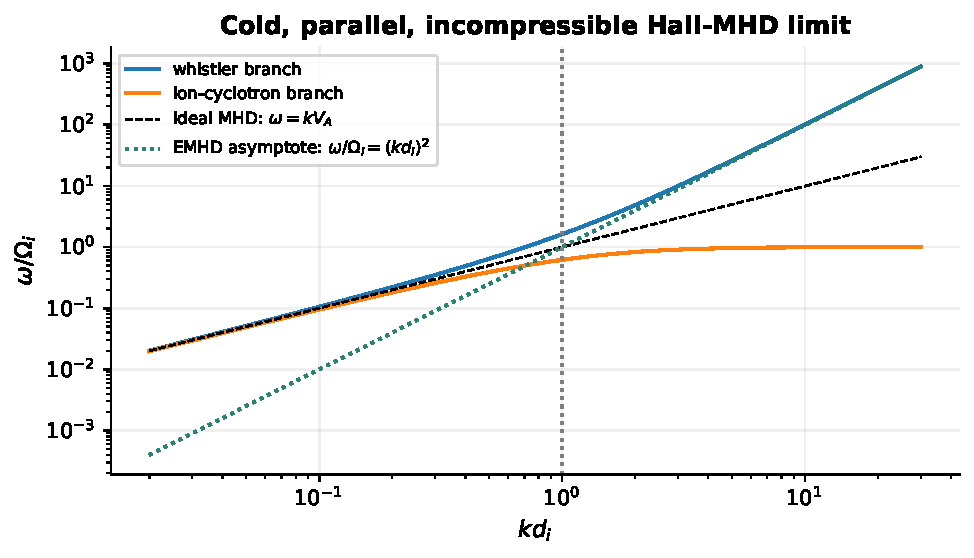
\includegraphics[width=.96\textwidth]{figures/06_dispersion.pdf}
\caption{由本章二次方程直接计算的两支色散关系，不是数值模拟拟合。$kd_i\ll1$时回到MHD；短波whistler频率随$k^2$增长，提示显式时间步会随网格变细而更严格。}\label{hall:figwave}\end{figure}

\worked{波长、波数和频率的完整换算}
仍取实验室教学参数。$d_i=0.072008$ m、$\Omega_i=4.7894\times10^6$ s$^{-1}$。
当$kd_i=0.1$时，$k=1.3887$ m$^{-1}$，$\lambda=2\pi/k=4.525$ m。两支$\omega_+/\Omega_i=0.105125$、$\omega_-/\Omega_i=0.095125$，故普通频率分别为80.1 kHz、72.5 kHz。它们相近，但并不完全相等。

当$kd_i=1$时，$\lambda=0.4525$ m，两个比值分别为1.6180和0.6180，频率分别为1.233 MHz和0.471 MHz。当$kd_i=10$时，$\lambda=4.525$ cm，whistler比值为100.990，频率约77.0 MHz；此时$kd_e=0.2334$，电子惯性修正已经不再极小。不要把$d_i$叫“波长”：$k d_i=1$对应的是$\lambda=2\pi d_i$，差一个$2\pi$。

\section{电子惯性如何限制无界的短波增长}
若进一步取固定离子、常密度、不可压电子流，保留电子惯性，可定义
\begin{equation}\B_e=\B-d_e^2\nabla^2\B.\end{equation}
在线性平行扰动中$\nabla^2\vct b_1=-k^2\vct b_1$，所以$\vct b_e=(1+d_e^2k^2)\vct b_1$，固定离子的whistler色散关系变为
\begin{equation}
|\omega|=\frac{C_Hk^2}{1+d_e^2k^2},\qquad
\lim_{kd_e\to\infty}|\omega|=\frac{C_H}{d_e^2}=|\Omega_e|.
\end{equation}
这不是前面完整离子响应色散关系在所有$k$上的精确替代式，而是另一组已说明近似的电子流体极限。它说明电子惯性不会永远容许无质量Hall模型的$k^2$频率增长。

在$kd_e\ll1$的whistler区，$v_{\rm ph}=\omega/k=C_Hk$，$v_g=\dd\omega/\dd k=2C_Hk$。包含上述电子惯性后，
\begin{equation}v_g=\frac{2C_Hk}{(1+d_e^2k^2)^2}.\end{equation}
色散让不同尺度以不同速度传播，能够改变重联层的通讯和形态，但这一线性波公式并未求解非线性层长、边界供能或破冻结，所以不能单凭它推导所有重联率等于某个常数。
